\chapter{绘制函数图像}
这里分享的是一个初学者制作的几个简单的数学象限里的图片

\begin{tikzpicture}[domain=-2:4,yscale=1,samples=200,>=latex,thick]
% \clip (0,0) rectangle (5,5);% 切り抜き
\draw[thick,->] (-1,0) -- (4,0) node[right] {$x$};% x軸
\draw[thick,->] (0,-1) -- (0,4) node[below left] {$y$};% y軸
\draw (0,0) node[below left] {O};% 原点

\coordinate (O) at (0,0);

\draw[domain=-0.5:2,color=black] plot (\x, {2*\x}) node[right] {$y=2x$};
\draw[domain=-1:4,color=black] plot (\x, {-2/3*\x+2}) node[right] {$2x+3y=6$};
\draw[domain=-1:4,color=black] plot (\x, {3/2}) node[right] {$y=\dfrac{3}{2}$};

\coordinate (A) at (1,2);
\coordinate (O) at (3/4,3/2);
\coordinate (B) at (2,3/2);
\coordinate (C) at (2,2/3);

\pic["$\alpha$",draw=black,->,very thick,angle eccentricity=1.4,angle radius=8mm] {angle=B--O--A};
\pic["$\beta$",draw=black,->,thick,angle eccentricity=1.4,angle radius=9mm] {angle=C--O--B};
\end{tikzpicture}
\begin{tikzpicture}[domain=-2:4,yscale=1,samples=200,>=latex,thick]
% \clip (0,0) rectangle (5,5);% 切り抜き
\draw[thick,->] (-2,0) -- (4,0) node[right] {$x$};% x軸
\draw[thick,->] (0,-2) -- (0,6) node[below left] {$y$};% y軸
\draw (0,0) node[below left] {O};% 原点

\draw (0,0) circle[radius=10mm];

\coordinate (O) at (0,0);
\coordinate (A) at (5/2,12/2);
\coordinate (B) at (4/2,-3/2);
\coordinate (C) at (77/65,21/65);

\fill (A) circle (2pt) node[right] {$\mathrm{A}(5,12)$};% 点
\fill (B) circle (2pt) node[right] {$\mathrm{B}(4,-3)$};% 点
\fill (C) circle (2pt) node[right] {$\mathrm{C}$};% 点

\draw (O)--(A);
\draw (O)--(B);
\draw (C)--(5/13,12/13);
\draw (C)--(4/5,-3/5);

\draw [thick,->] (O)--(5/13,12/13) node[right] {$\dfrac{\bm{a}}{\|\bm{a}\|}$};
\draw [thick,->] (O)--(4/5,-3/5) node[right] {$\dfrac{\bm{b}}{\|\bm{b}\|}$};

\draw[domain=-2:3,color=black] plot (\x, {3/11*\x}) node[right] {$3x-11y=0$};
\end{tikzpicture}


\begin{tikzpicture}[domain=-2:4,yscale=0.5,samples=200,>=latex,thick]
% \clip (0,0) rectangle (5,5);% 切り抜き
\draw[thick,->] (-2,0) -- (4,0) node[right] {$x$};% x軸
\draw[thick,->] (0,-4) -- (0,7) node[below right] {$y$};% y軸
\draw (0,0) node[below left] {O};% 原点
\draw[domain=-2:-0.36,color=black] plot (\x, {(2*\x*\x*\x+1)/(\x*\x)}) node[below left] {$y=\dfrac{2x^3+1}{x^2}$};
\draw[domain=0.4:3,color=black] plot (\x, {(2*\x*\x*\x+1)/(\x*\x)});
\draw[domain=-2:3,color=black,dashed,thin] plot (\x, {2*\x});
\draw (1.2,2) node[right] {$y=2x$};
\draw[domain=-2:4,color=black] plot (\x, {-2}) node[below] {$y=a$};
\end{tikzpicture}
\begin{tikzpicture}[domain=-2:4,scale=1,samples=200,>=latex,thick]
% \clip (0,0) rectangle (5,5);% 切り抜き
\draw[thick,->] (-2,0) -- (5,0) node[right] {$x$};% x軸
\draw[thick,->] (0,-1) -- (0,9) node[below right] {$y$};% y軸
\draw (0,0) node[below left] {O};% 原点

\draw[domain=4.2:-2.5,color=black] plot (\x, {1/2*\x*\x}) node[right] {$C:y=\dfrac{1}{2}x^2$};
\draw[domain=-0.5:4.4,color=black] plot (\x, {2*\x}) node[right] {$y=2x$};

\coordinate (O) at (0,0);
\coordinate (Q) at (2,2);
\coordinate (R) at (2,4);
\coordinate (P) at (1*1.2,2*1.2);

\draw[dashed] (4,8) -- (4,0) node[below] {4};% y軸

\draw (Q) node[right] {Q};
\draw (R) node[above left] {R};
\draw (P) node[left] {P};
\draw (2,0) node[below] {$t$};

\draw (R)--(2,0);
\draw (O)--(P) node [midway,left] {$X$};
\draw (P)--(Q) node [midway,below] {$Y$};

\draw [bend left,distance=20mm,dotted] (O) to node [fill=white,inner sep=0.5pt,circle] {[$\sqrt{5}$]} (R);
\draw [bend right,distance=10mm,dotted] (O) to node [fill=white,inner sep=0.5pt,circle] {[1]} (2,0);
\draw [bend left,distance=20mm,dotted] (R) to node [fill=white,inner sep=0.5pt,circle] {[2]} (2,0);
\end{tikzpicture}


\begin{tikzpicture}[domain=-2:4,scale=0.5,samples=200,>=latex,thick]
% \clip (0,0) rectangle (5,5);% 切り抜き
\draw[thick,->] (-2,0) -- (10,0) node[right] {$x$};% x軸
\draw[thick,->] (0,-1) -- (0,9) node[below right] {$y$};% y軸
\draw (0,0) node[below left] {O};% 原点

\draw[domain=4.2:-2.5,color=black] plot (\x, {1/2*\x*\x}) node[right] {$C:y=\dfrac{1}{2}x^2$};
\draw[fill=black] (2,2) circle[radius=1mm] node[right] {$P$};
\draw[domain=4.2:-1.5,color=black,rotate=-63] plot (\x, {1/2*\x*\x});
\draw[fill=black,rotate=-63] (2,2) circle[radius=0.8mm] node[below] {$P'$};

\draw[domain=-0.5:4.4,color=black] plot (\x, {2*\x}) node[right] {$y=2x$};

\draw[dashed] (4,8) -- (4,0) node[below] {4};% y軸
\draw (8.8,0) node[below] {$4\sqrt{5}$};
\draw (0.2,0) node[above right] {$\theta$};

\coordinate (O) at (0,0);

\draw [bend left,distance=20mm,dotted] (O) to node [fill=white,inner sep=0.5pt,circle] {[$\sqrt{5}$]} (4,8);
\draw [bend left,distance=20mm,dotted] (4,8) to node [fill=white,inner sep=0.5pt,circle] {[2]} (4,0);
\draw [bend left,distance=15mm,dotted] (O) to node [fill=white,inner sep=0.5pt,circle] {[1]} (4,0);
\end{tikzpicture}